% Insert result section here. 
\section{Results}
\label{sec:Results}
Some text
%%%%%%%%%%%%%%% XY %%%%%%%%%%%%%%%%%%%%%%%%%

\begin{figure}[htb]
  \begin{center}
    \begin{subfigure}[b]{0.4\textwidth}
      \centering
      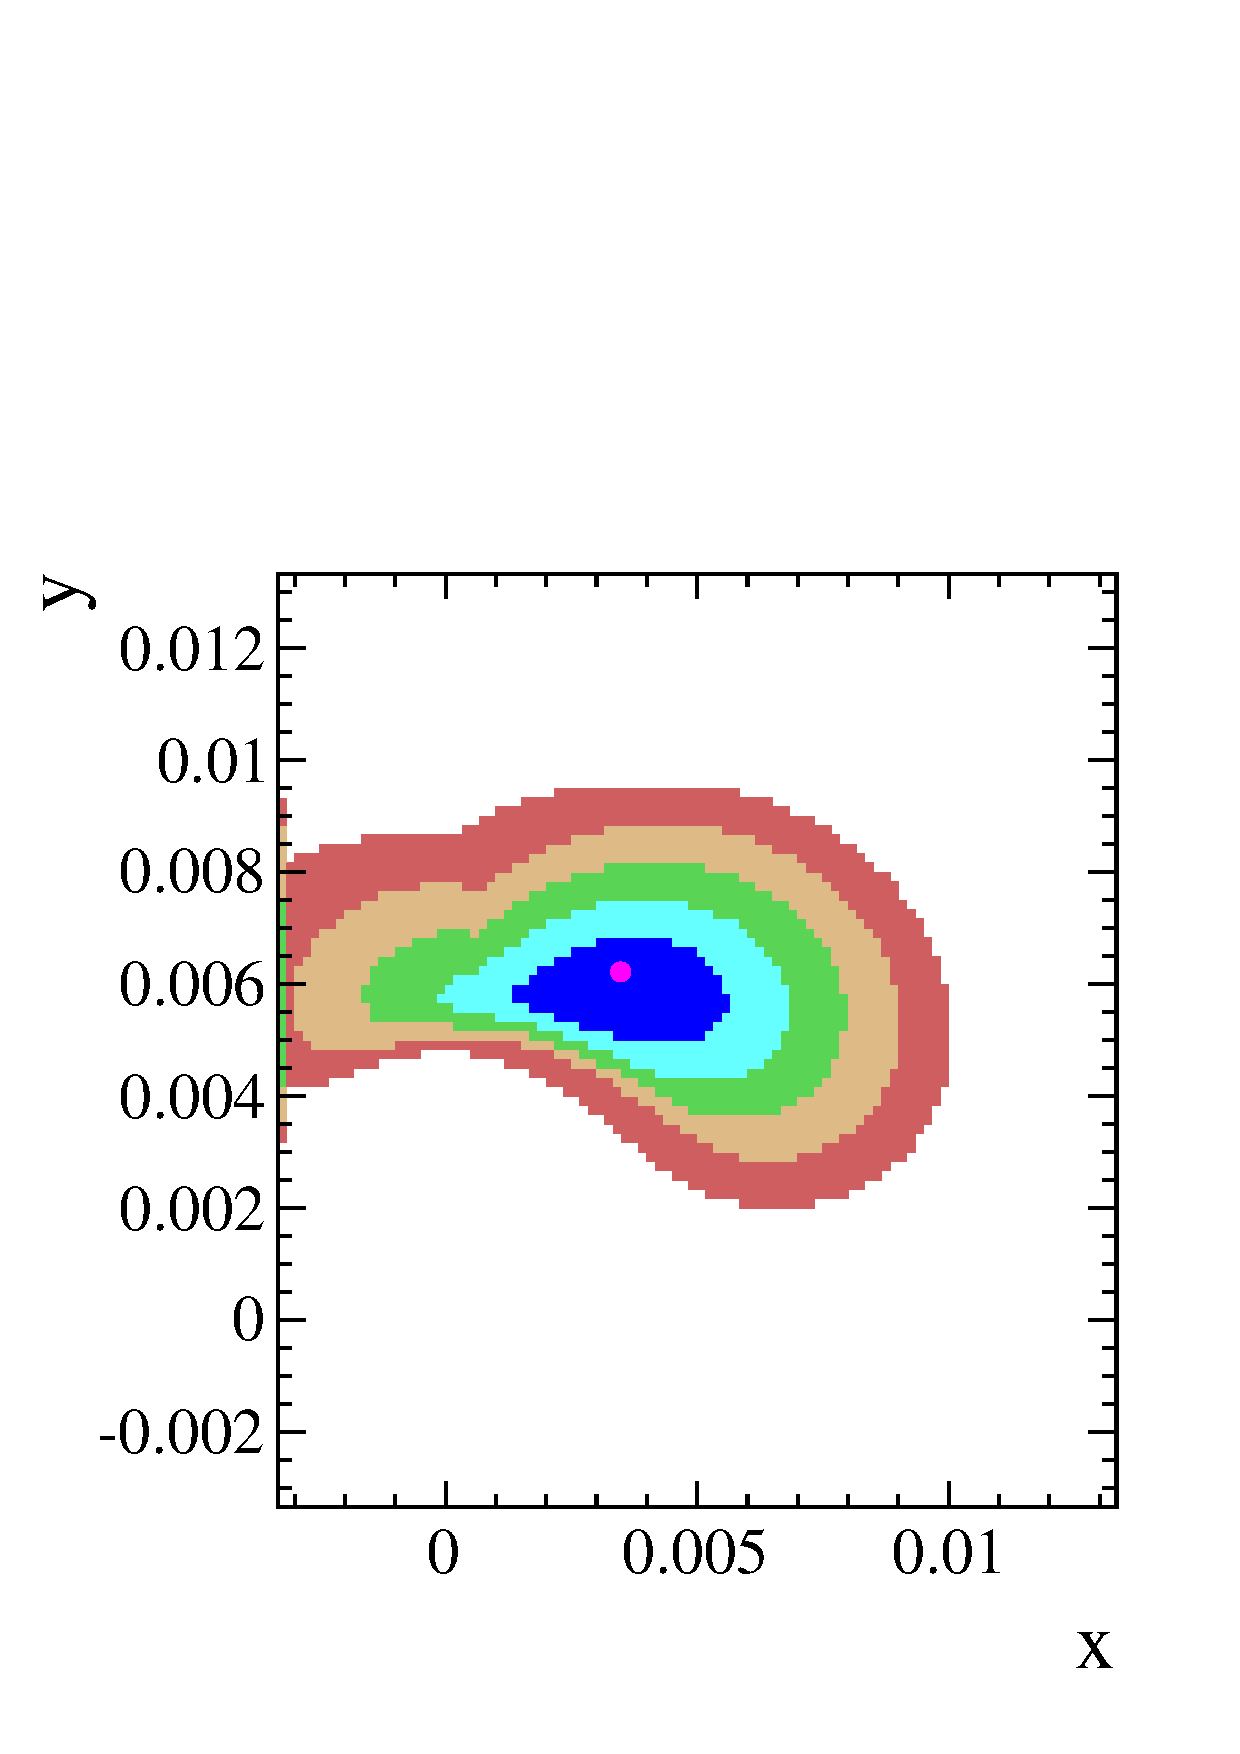
\includegraphics[width=\textwidth]{./output/finalplot_allcpv_no_belle_babar_graph_hfag_agamma.pdf}
      \caption{Two dimensional error ellipses for x and y from fit excluding Belle and BaBar $K\pi$ results. Does not include latest $A_\Gamma$ result of LHCb.}
      \label{fig:xy_all_cpv_no_agamma}
    \end{subfigure}%
    \hspace{2mm}
    \begin{subfigure}[b]{0.4\textwidth}
      \centering
      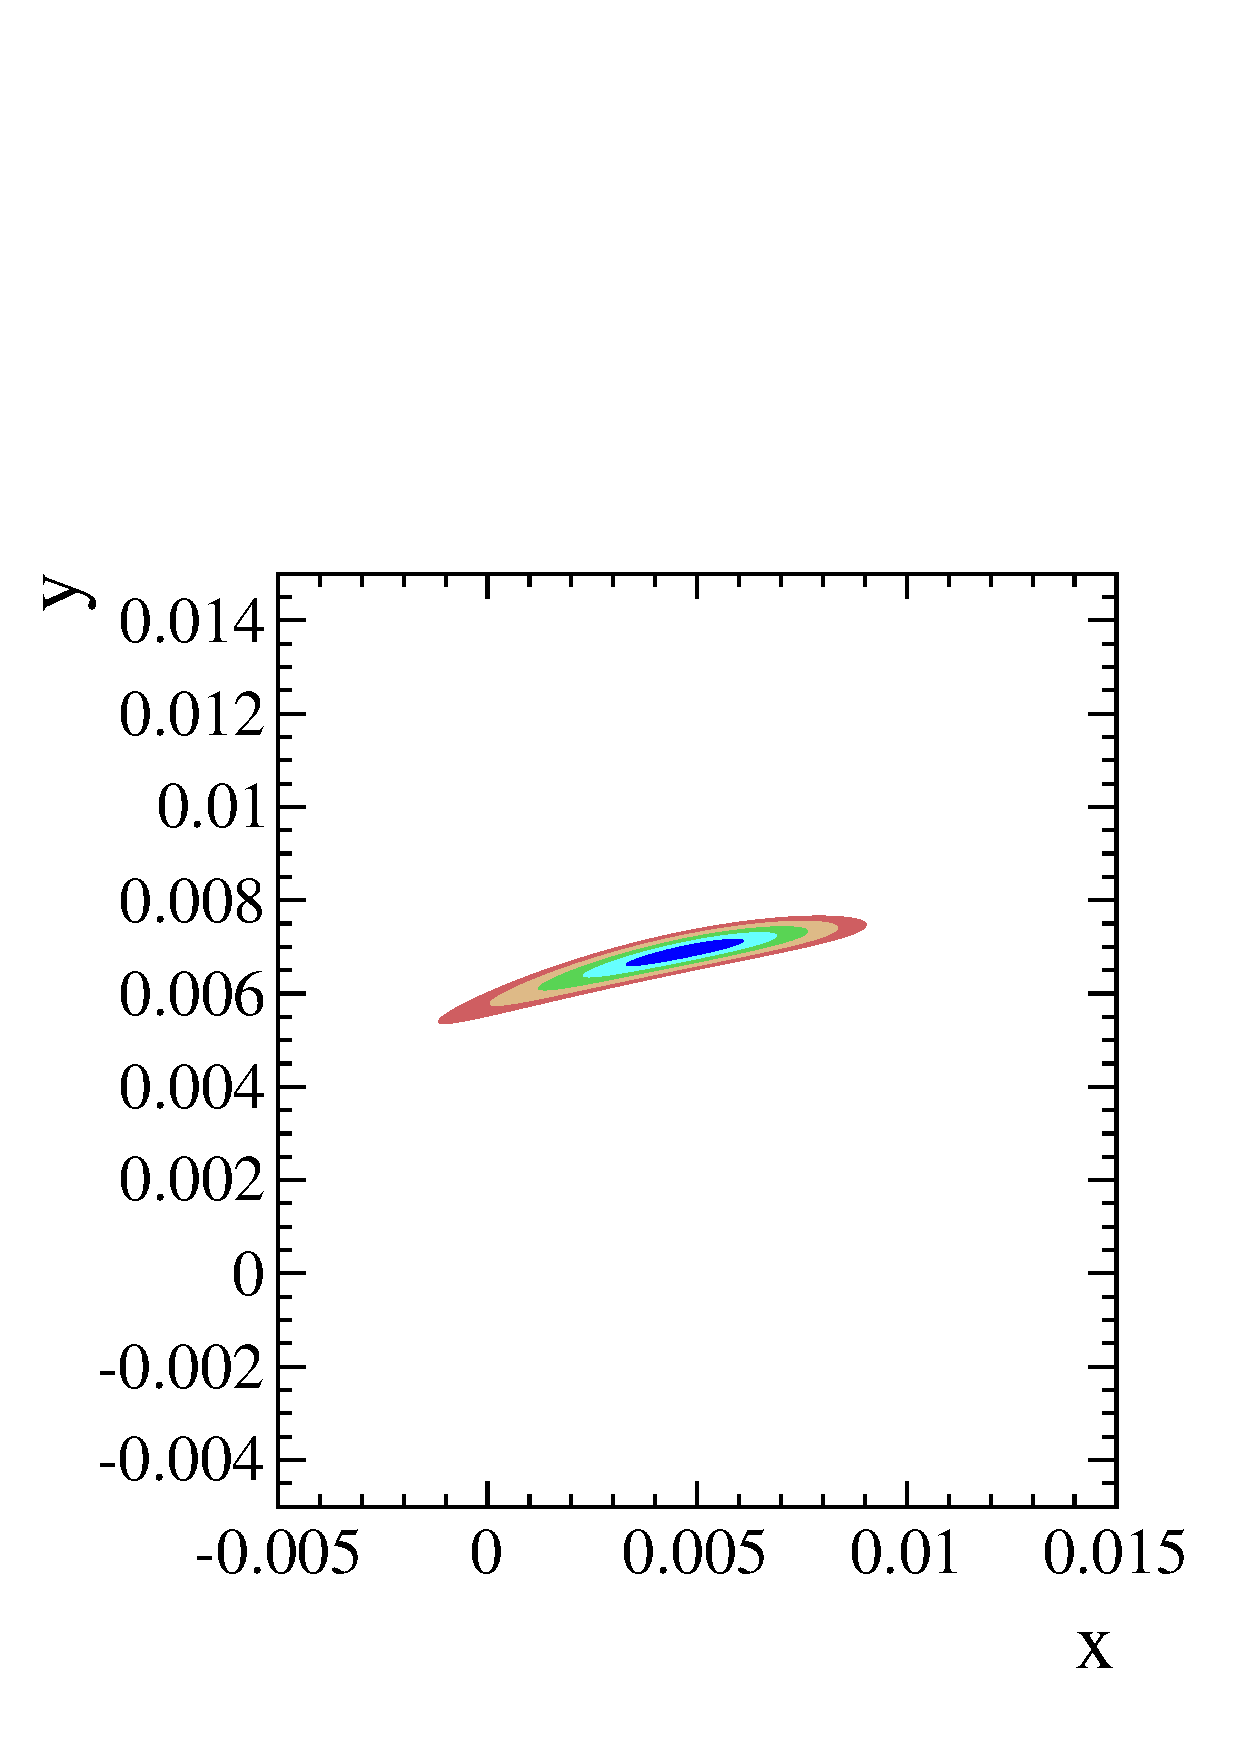
\includegraphics[width=\textwidth]{./output/finalplot_allcpv_no_belle_babar_graph_lhcb_agamma.pdf}
      \caption{Two dimensional error ellipses for x and y from fit excluding Belle and BaBar $K\pi$ results. Include latest $A_\Gamma$ result of LHCb.}
      \label{fig:xy_all_cpv_with_agamma}
    \end{subfigure}%
    \\
%%%%%%%%%
    %\hspace{2mm}
    \begin{subfigure}[b]{0.4\textwidth}
      \centering
      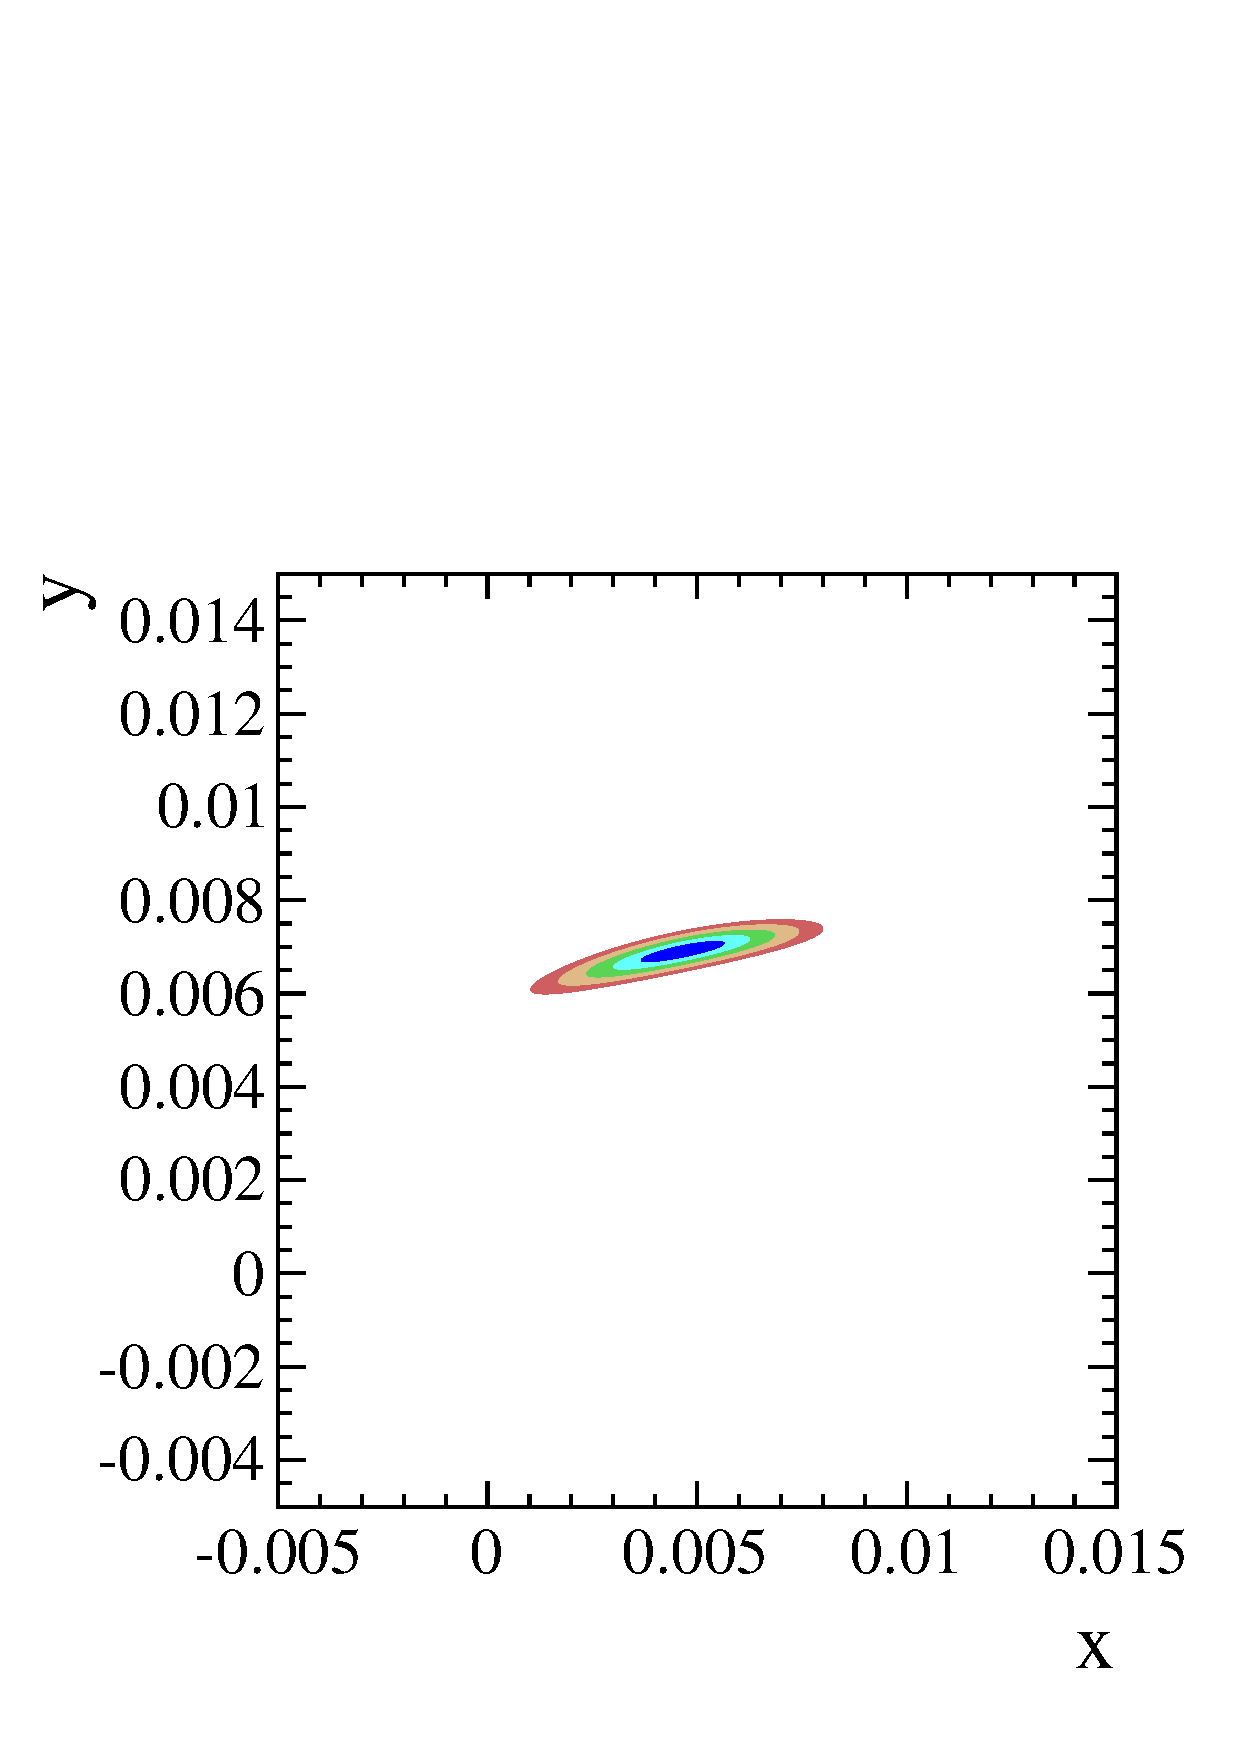
\includegraphics[width=\textwidth]{./output/finalplot_allcpv_no_belle_babar_cdf_graph_hfag_agamma.pdf}
      \caption{Two dimensional error ellipses for x and y from fit excluding Belle, BaBar and CDF $K\pi$ results. Does not include latest $A_\Gamma$ result of LHCb.}
      \label{fig:xy_all_cpv_no_agamma}
    \end{subfigure}%
    \hspace{2mm}
    \begin{subfigure}[b]{0.4\textwidth}
      \centering
      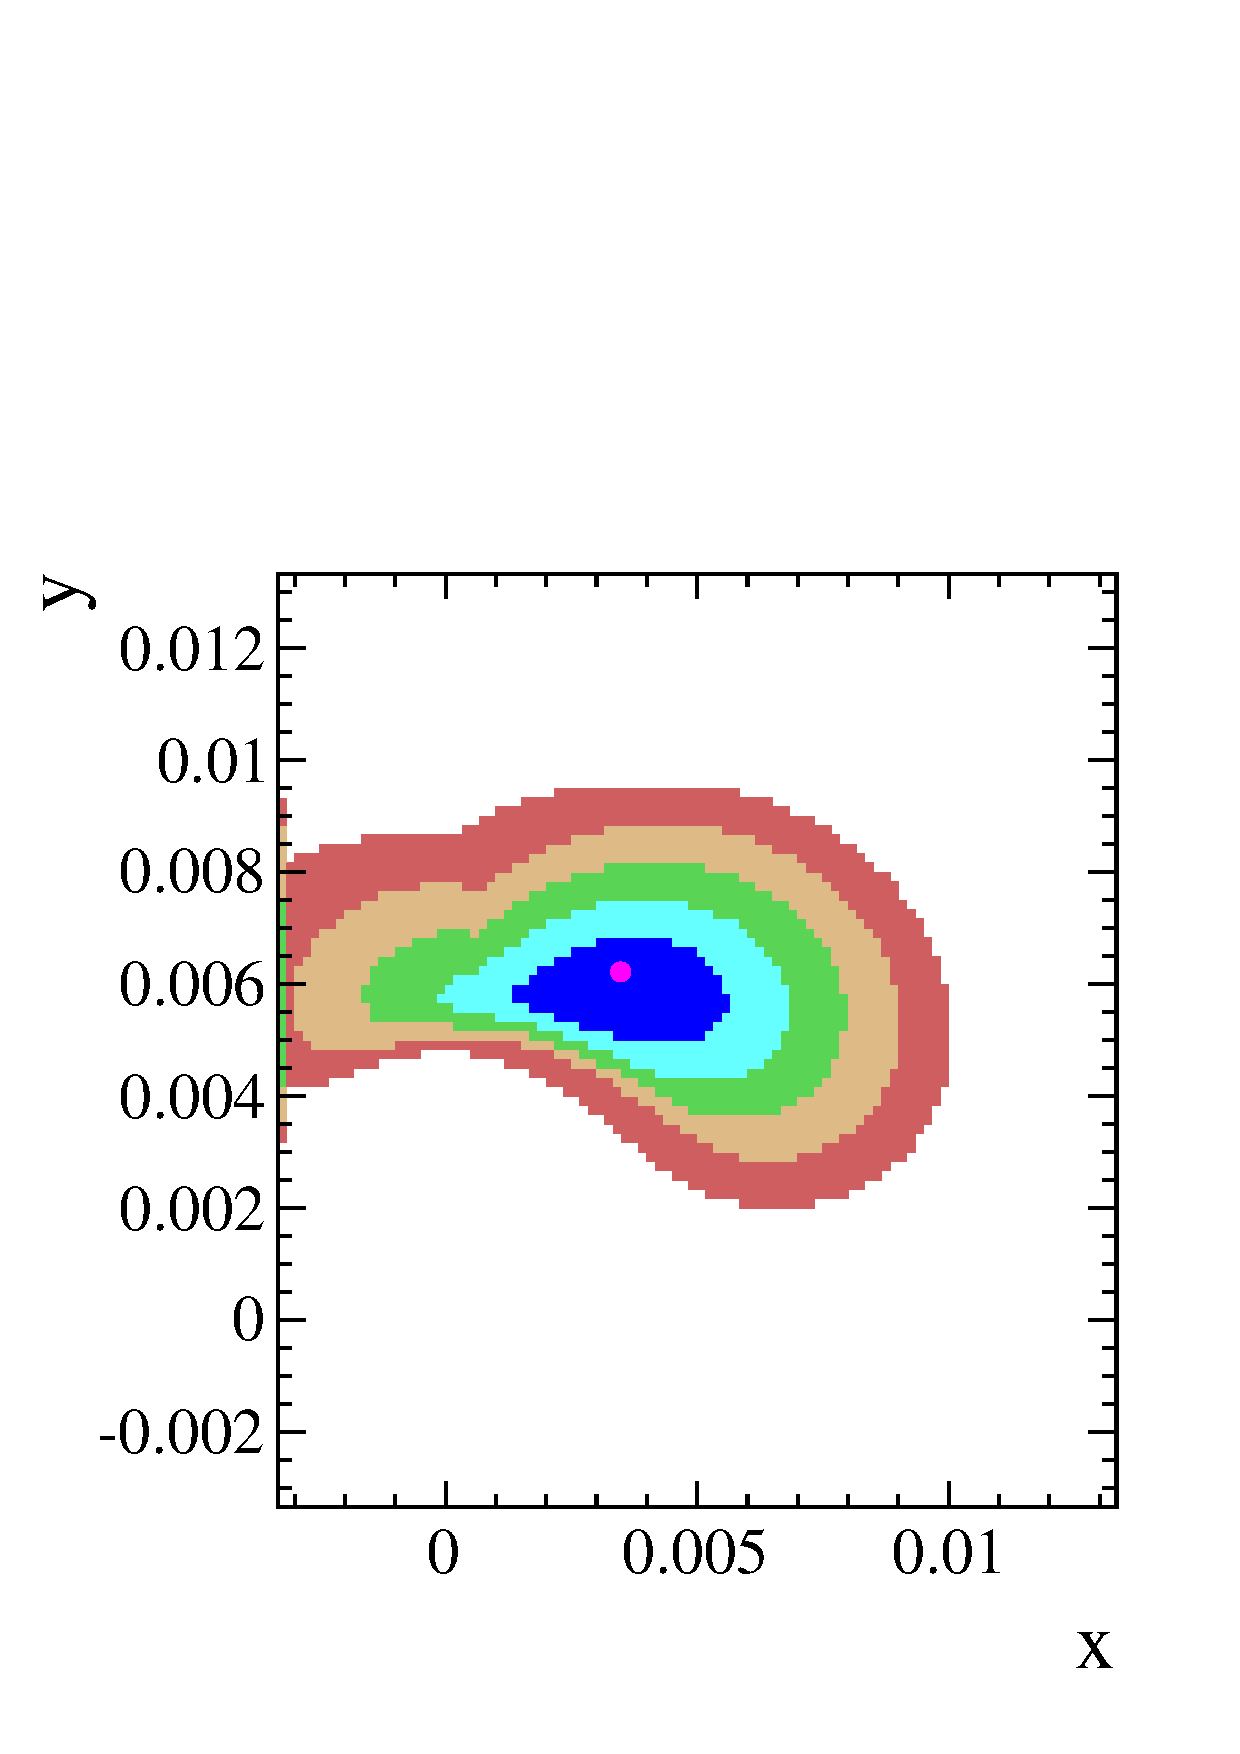
\includegraphics[width=\textwidth]{./output/finalplot_allcpv_no_belle_babar_cdf_graph_lhcb_agamma.pdf}
      \caption{Two dimensional error ellipses for x and y from fit excluding Belle, BaBar and CDF $K\pi$ results. Include latest $A_\Gamma$ result of LHCb.}
      \label{fig:xy_all_cpv_with_agamma}
    \end{subfigure}%
    %\vspace*{-1.0cm}
  \end{center}
  \caption{Two dimensional error ellipses of fit for All CPV including differing sets of data for $x$ vs $y$. The biggest differences come from including the CDF result, which elongates the error ellipses. The differing colors represent the 1-5$\sigma$ contours.}
  \label{fig:xy_all_variations}
\end{figure}

%%%%%%%%%%%%%%%% Q/P %%%%%%%%%%%%%%%%%%%%%%%%%%%%%%%%%%%%
\begin{figure}[tb]
  \begin{center}
    \begin{subfigure}[b]{0.4\textwidth}
      \centering
      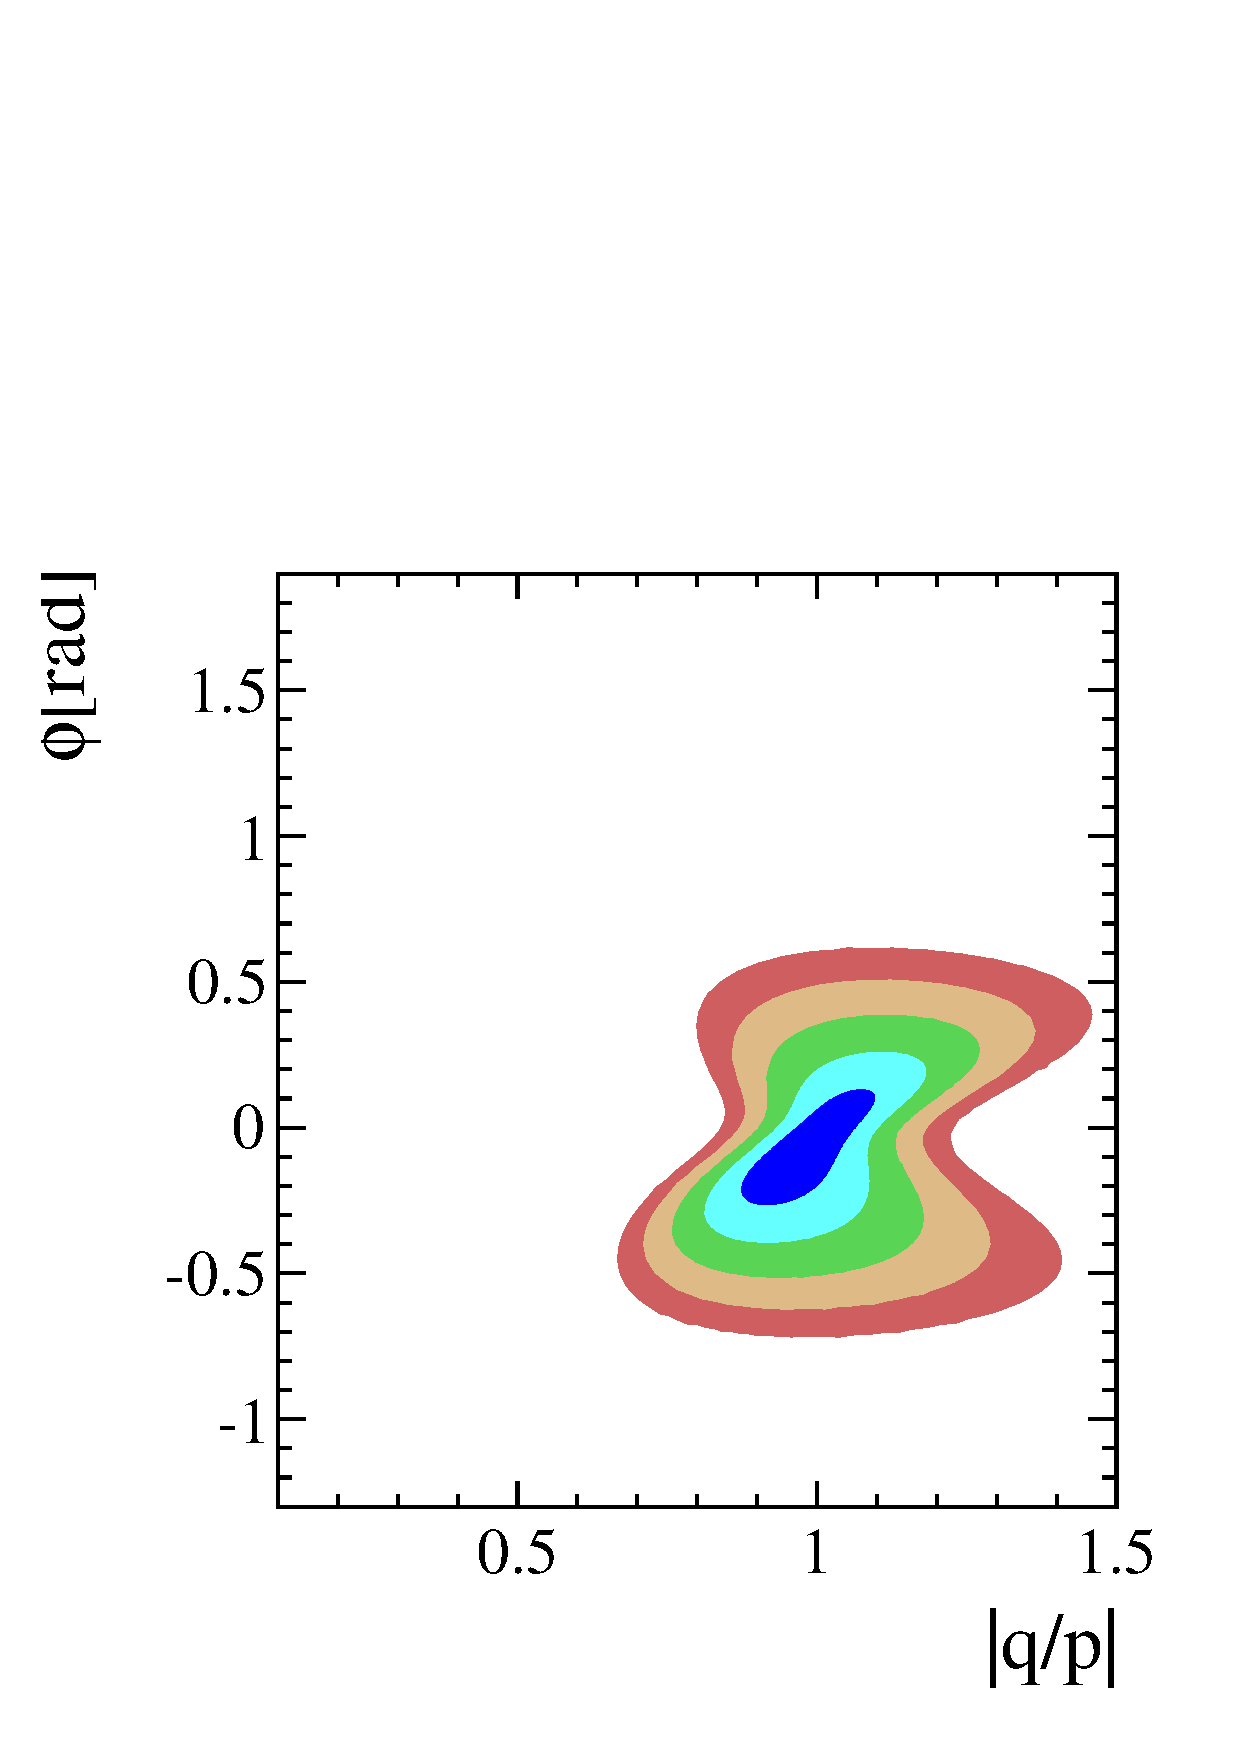
\includegraphics[width=\textwidth]{./output/finalplot_allcpv_no_belle_babar_graph_qop_phi_hfag_agamma.pdf}
      \caption{Two dimensional error ellipses for x and y from fit excluding Belle and BaBar $K\pi$ results. Does not include latest $A_\Gamma$ result of LHCb.}
      \label{fig:xy_all_cpv_no_agamma}
    \end{subfigure}% 
    \hspace{2mm}
    \begin{subfigure}[b]{0.4\textwidth}
      \centering
      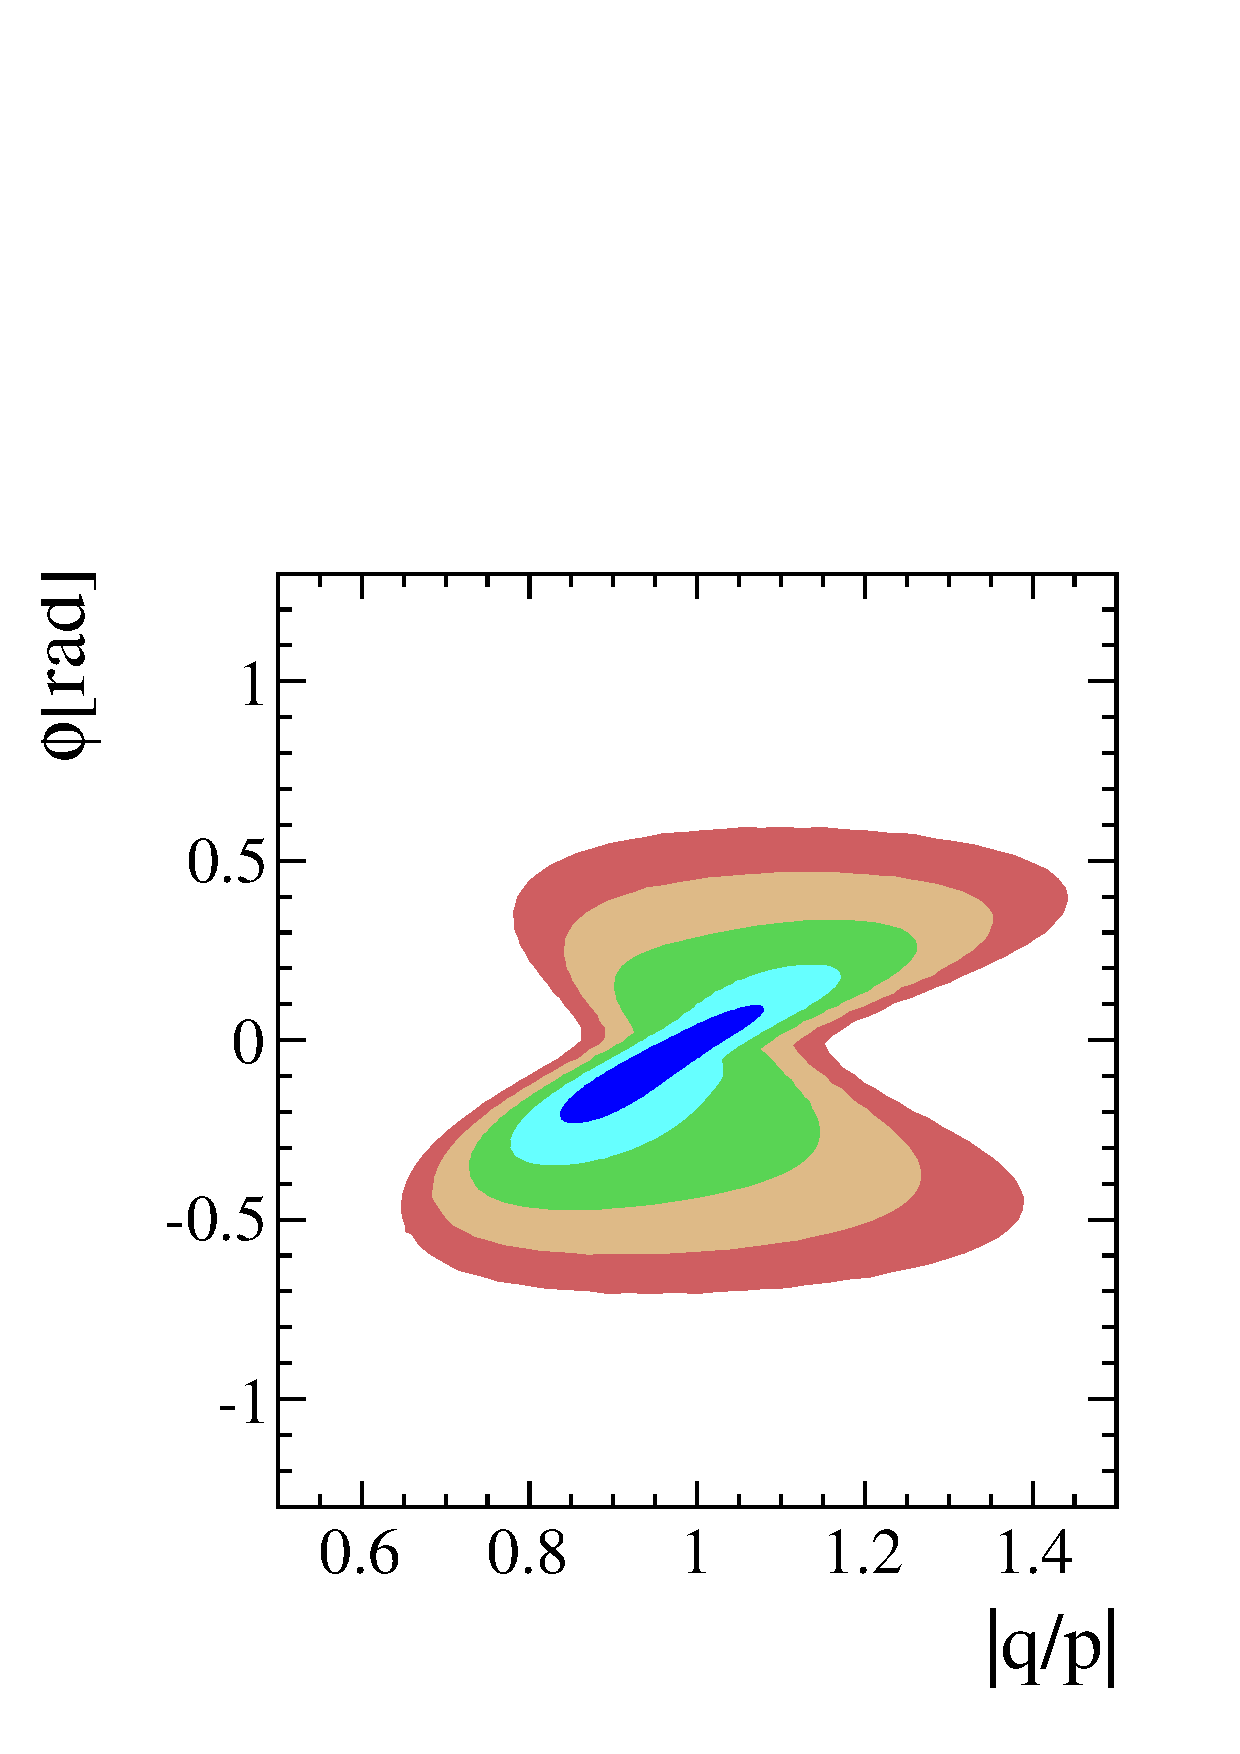
\includegraphics[width=\textwidth]{./output/finalplot_allcpv_no_belle_babar_graph_qop_phi_lhcb_agamma.pdf}
      \caption{Two dimensional error ellipses for x and y from fit excluding Belle and BaBar $K\pi$ results. Include latest $A_\Gamma$ result of LHCb.}
      \label{fig:xy_all_cpv_with_agamma}
    \end{subfigure}%
%%%%%%%%%
        \\
    \begin{subfigure}[b]{0.4\textwidth}
      \centering
      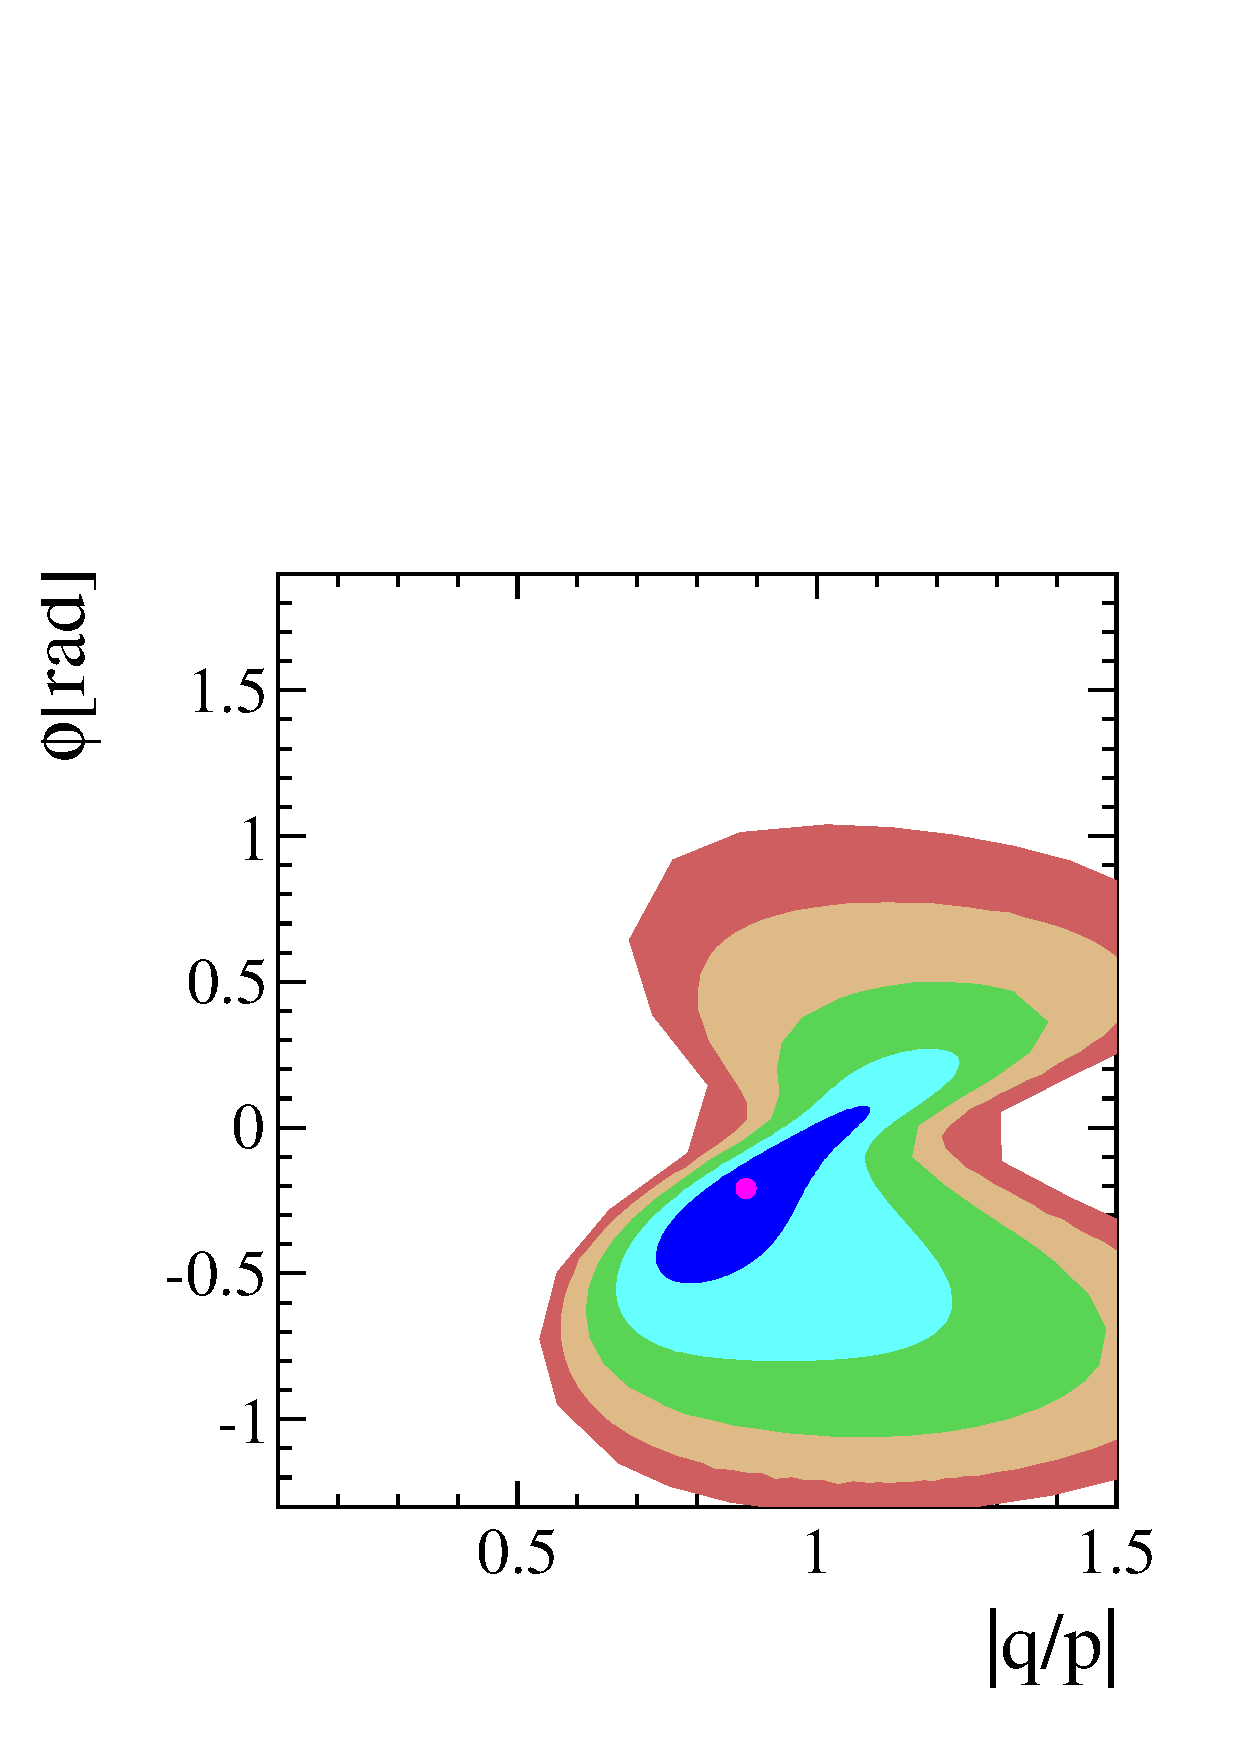
\includegraphics[width=\textwidth]{./output/finalplot_allcpv_no_belle_babar_cdf_graph_qop_phi_hfag_agamma.pdf}
      \caption{Two dimensional error ellipses for x and y from fit excluding Belle, BaBar and CDF $K\pi$ results. Does not include latest $A_\Gamma$ result of LHCb.}
      \label{fig:xy_all_cpv_no_agamma}
    \end{subfigure}%
    \hspace{2mm}
    \begin{subfigure}[b]{0.4\textwidth}
      \centering
      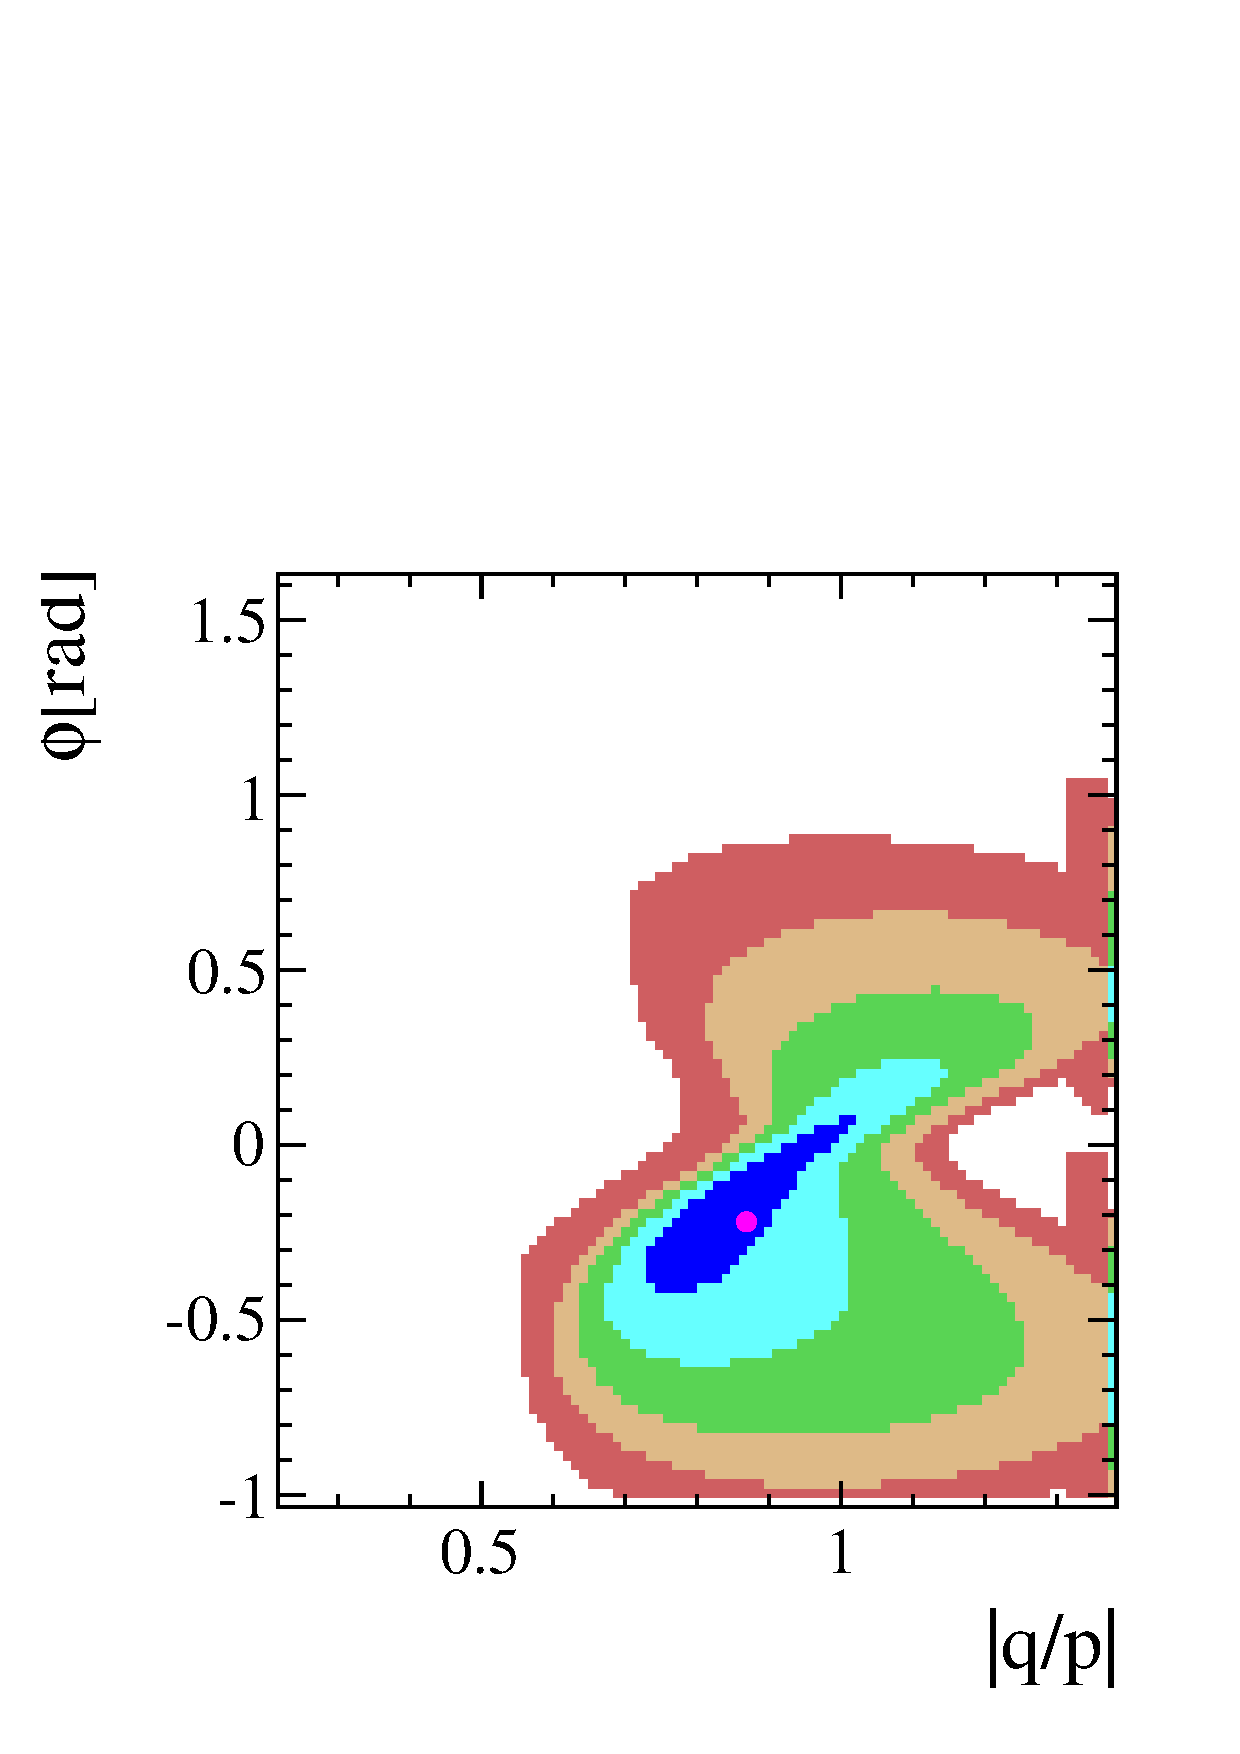
\includegraphics[width=\textwidth]{./output/finalplot_allcpv_no_belle_babar_cdf_graph_qop_phi_lhcb_agamma.pdf}
      \caption{Two dimensional error ellipses for x and y from fit excluding Belle, BaBar and CDF $K\pi$ results. Include latest $A_\Gamma$ result of LHCb.}
      \label{fig:xy_all_cpv_with_agamma}
    \end{subfigure}%
    %\vspace*{-1.0cm}
  \end{center}
  \caption{Two dimensional error ellipses of fit for All CPV including differing sets of data for $x$ vs $y$. The biggest differences come from including the CDF result, which elongates the error ellipses. The differing colors represent the 1-5$\sigma$ contours.}
  \label{fig:xy_all_variations}
\end{figure}
